%!TEX root = ../report_nips.tex
\subsection{n-Grams} % (fold)
\label{sub:n_grams}

N-Grams are one of the most used features in NLP as they can be used to describe meaningful collections of words - a desirable trait for many contexts. Formally an n-gram is a contiguous sequence of $n$ items taken from a larger sequence. In the context of NLP, a n-gram can take on the form of $n$ characters, syllables, words, or even phonemes.

	To best understand how meaning can be translated in a n-gram lets consider an example. A unigram is a n-gram for $n = 1$. This is the most basic n gram where you consider each item separately. In our application unigrams form the base features, and are actually the most important features in our pipeline. As an example, a tweet such as: “I hate work” would generate three features, (“I”), (“hate”), and (“work”). In the context of sentiment analysis the individual words can carry sentiment, as such the feature (“hate”) can be an important feature to predict the sentiment of the whole tweet. 

	Bigrams are the next n-gram we explored, where $n = 2$. These features are all sequence pairings or words in a tweet. Again with the example: “I hate work”, we would generate two bigrams: (“I hate”) and (“hate work”). The intuition behind using bigrams as a feature is that bigrams like (“I hate”) carry a different sentiment value than simple the words separately. Additionally, words that don’t necessarily communicate sentiment by themselves would carry sentiment when considered together, such as (“this sucks”).

	N-grams with $n \geq 3$ are not considered as the number of unique trigrams and above combinatorially explode. Here we can imagine trigrams carry unique sentiment again, but its difficult for our algorithm to pick this up as the frequency of such trigrams is low and we don’t hand pick which ones we think would work best.

	To build a feature vector from a set of documents all containing a set of n-grams we add each gram to a bag of words dictionary. Then when a feature vector is created for a tweet we look up the unique place within that dictionary for each gram in order to determine which dimension to increment the count of that gram. 

	In building our feature vectors we only considered the frequency of the grams, instead of the just the 0/1 presence or the td-idf (term frequency-inverse document frequency). In doing this our n-gram implementation can also be used to pick up and count the number of special tokens we have inserted such as special mapped tokens from preprocessing, and POS tags.

% subsection n_grams (end)

\subsection{Part of Speec (POS) Tagging} % (fold)
\label{sub:part_of_speec_}

One of the most fundamental parts of the linguistic pipeline is the part-of-speech (POS) tagging, a basic form of syntactic analysis which has countless applications in Natural Language Processing (NLP). We studied some of the best POS tagging tools \& settled on using Tweet NLP, a twitter specific POS tagger. We’ve used part-of-speech tagging as a feature for our task wherein every word/token in a given tweet is tagged based on its part-of-speech, some of which are twitter specific.

\begin{figure}[ht]
\centering 
  \begin{tabular}{@{}l@{}}
    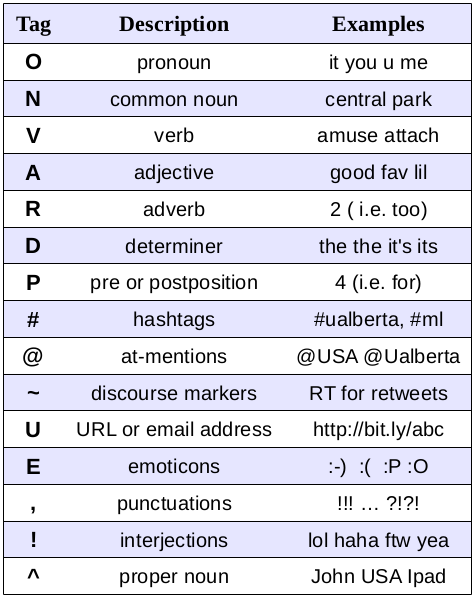
\includegraphics[width=0.4\linewidth]{img/tags-final.png}
  \end{tabular} 
  \caption{caption msdbkjsghsg} 
  \label{fig:tags_final} 
\end{figure}

\begin{table}[t]
\caption{Sample table title}
\label{sample-table}
\begin{center}
\begin{tabular}{lll}
\multicolumn{1}{c}{\bf TAG}  &\multicolumn{1}{c}{\bf DESCRIPTION} &\multicolumn{1}{c}{\bf EXAMPLES}
\\ \hline \\
O & pronoun & it you u me \\
N & common noun & central park\\
V & verb & amuse attach\\
A & adjective & good fav lil\\
R & adverb & 2 ( i.e. too)\\
D & determiner & the the it's its\\
P & pre or postposition & 4 (i.e. for)\\
\# & hashtags & \#ualberta, \#ml\\
@ & at-mentions & @USA @Ualberta\\
\textasciitilde & discourse markers & RT for retweets\\
U & URL or email address & http://bit.ly/abc\\
E & emoticons & :-) :( :P :O\\
, & punctuations & !!! \dots ?!?!\\
! & interjections & lol haha ftw yea\\
\textasciicircum & proper noun & John USA Ipad\\
\end{tabular}
\end{center}
\end{table}

For our task, we selected 15 of the most common tags in linguistics (including the twitter specific tags). we made a count of the number of tagged tokens (with a confidence score > 0.9) in a tweet \& then used that as a feature.[rough work]

% subsection part_of_speec_ (end)

\subsection{Sentiment} % (fold)
\label{sub:sentiment}

We used \textit{SentiWordNet} to add features specifically related to the sentiment of the tweets. This is dictionary, designed for opinion mining, where each of the over 100,000 words is assigned a positive and negative sentiment score. For a given tweet, we calculate a positive sum feature: $p_{sum} = \sum_{i}^n p_i$ , where piis the positive sentiment score from SentiWordNet for the ith word in a tweet with n words. We similarly calculate a negative sum feature. If a word is not found in the dictionary, then it does not contribute to either of the two sentiment features. These two features are added to the bag of words feature vector as a real number. It is possible that different preprocessing steps could affect the sentiment score of a tweet by modifying said tweet (such as by stemming); future experimentation is required to determine the effects of different combinations of preprocessing on sentiment score.

% subsection sentiment (end)

\subsection{Irony} % (fold)
\label{sub:irony}

To account for possible irony in the tweets we implement two features based on the work of Reyes et. al [year]. The features are created to detect the so-called \textit{counter-factuality} and \textit{temporal compression} of a tweet. Reyes et. al. determined that ironic tweets were more likely to have a high level of these two measures.

\paragraph{Counter-factuality:} % (fold)
\label{par:counter_factuality_}
The first measure, counter-factuality, is focused on ``discursive terms that hint at opposition or contradiction in a text, such as about, nevertheless, nonetheless, and yet.'' (Citation). The full list of counter-factual words includes 41 entrees; there are a total of 4187 occurrences of these words in the data set, and 3123 tweets contain at least one counter-factual word.
% paragraph counter_factuality_ (end)

\paragraph{Temporal Compression:} % (fold)
\label{par:temporal_compression_}
The second measure of tweet irony that we considered is temporal compression, which focuses on words related to an opposition in time, thus indicating an abrupt change in narrative. (citation) The list of temporal compression words contains 13 words such as suddenly, abruptly, and now. There are only 170 instances of a temporal compression word in the dataset, with only 103 tweets even containing a single instance.
% paragraph temporal_compression_ (end)

\paragraph{Feature Creation:} % (fold)
\label{par:feature_creation_}
For each measure, we create a real-numbered feature based on the ratio of how many words in a given tweet possess the characteristic we are analyzing. That is, we have two ratio features $r_t = \frac{n_t}{n}$, where $t \in \left \{\ex{counterFactuality}, \ex{temporalCompression}\right \}$, $n_t$ is the number of words in a given tweet that fit into category $t$, and $n$ is the total number of words in the tweet.
% paragraph feature_creation_ (end)

% subsection irony (end)